\documentclass[a4paper,11pt]{article}

\usepackage[utf8]{inputenc}
\usepackage[T2A]{fontenc}
\usepackage[russian]{babel}
\usepackage{PTSans}
\renewcommand{\familydefault}{\sfdefault}
\usepackage{geometry}
\usepackage{graphicx}
\usepackage{xcolor}
\usepackage{hyperref}
\usepackage{multicol}

\geometry{top=1.0cm, bottom=1.0cm, left=1.4cm, right=1.4cm}

\definecolor{linkblue}{HTML}{4675D5}

\hypersetup{
  colorlinks=true,
  linkcolor=linkblue,
  urlcolor=linkblue,
  pdfborder={0 0 0}
}

\setlength{\parindent}{0pt}
\setlength{\parskip}{0pt}
\setlength{\columnsep}{16pt}

\newlength{\cvsectionsep}
\setlength{\cvsectionsep}{4pt}

\newcommand{\cvsection}[1]{%
  \vspace{5pt}%
  \noindent
  \begin{minipage}{\linewidth}
    \hrule height 0.4pt
    \vspace{\cvsectionsep}
    \hbox to \linewidth{\textbf{\MakeUppercase{#1}}\hss}
    \vspace{\cvsectionsep}
    \hrule height 0.4pt
  \end{minipage}%
  \par\vspace{3pt}%
}

\newcommand{\cvskill}[2]{%
  {\raggedright\noindent\textbf{#1} #2\par}
}

\newcommand{\cvprojecttitle}[2]{%
  \vspace{2pt}%
  \noindent\textbf{\MakeUppercase{#1}}\hfill\href{#2}{\textcolor{linkblue}{ссылка}}\par
  \vspace{1pt}%
}

\newcommand{\cvprojectbody}[2]{%
  \noindent #1\par
  \vspace{1pt}%
  \noindent\textbf{Стек:} #2\par
  \vspace{2pt}%
}

\newcommand{\cvproject}[4]{%
  \cvprojecttitle{#1}{#2}%
  \cvprojectbody{#3}{#4}%
}

\newcommand{\cvjob}[3]{%
  \vspace{2pt}%
  \noindent\textbf{\MakeUppercase{#1}}\par
  \vspace{1pt}%
  \noindent\textbf{Место:} #2\par
  \noindent\textbf{Задачи:} #3\par
  \vspace{2pt}%
}

\newcommand{\cvpractice}[3]{%
  \vspace{2pt}%
  \noindent\textbf{#1}\par
  #2\par
  #3\par
  \vspace{3pt}%
}

\newcommand{\cvheader}{%
  \noindent
  \begin{minipage}[t]{0.72\textwidth}
    \vspace{0pt}%
    {\fontsize{16}{18}\selectfont\textbf{БЕЛЯКОВА АННА СТАНИСЛАВОВНА}}\par
    \vspace{4pt}
    \textbf{СИСТЕМНЫЙ АНАЛИТИК}\par
    \vspace{30pt}
    +79877288420\,|\,20.07.2005\,|\,\href{https://t.me/belyak_anya}{t.me/belyak\_anya}\par
    belyakova.anna.st@yandex.ru\,|\,\href{https://github.com/belyakova-anna}{github}\,|\,\href{https://www.linkedin.com/in/belyak-anya/}{linkedin}\par
  \end{minipage}%
  \hfill
  \begin{minipage}[t]{0.22\textwidth}
    \vspace{0pt}%
    \raggedleft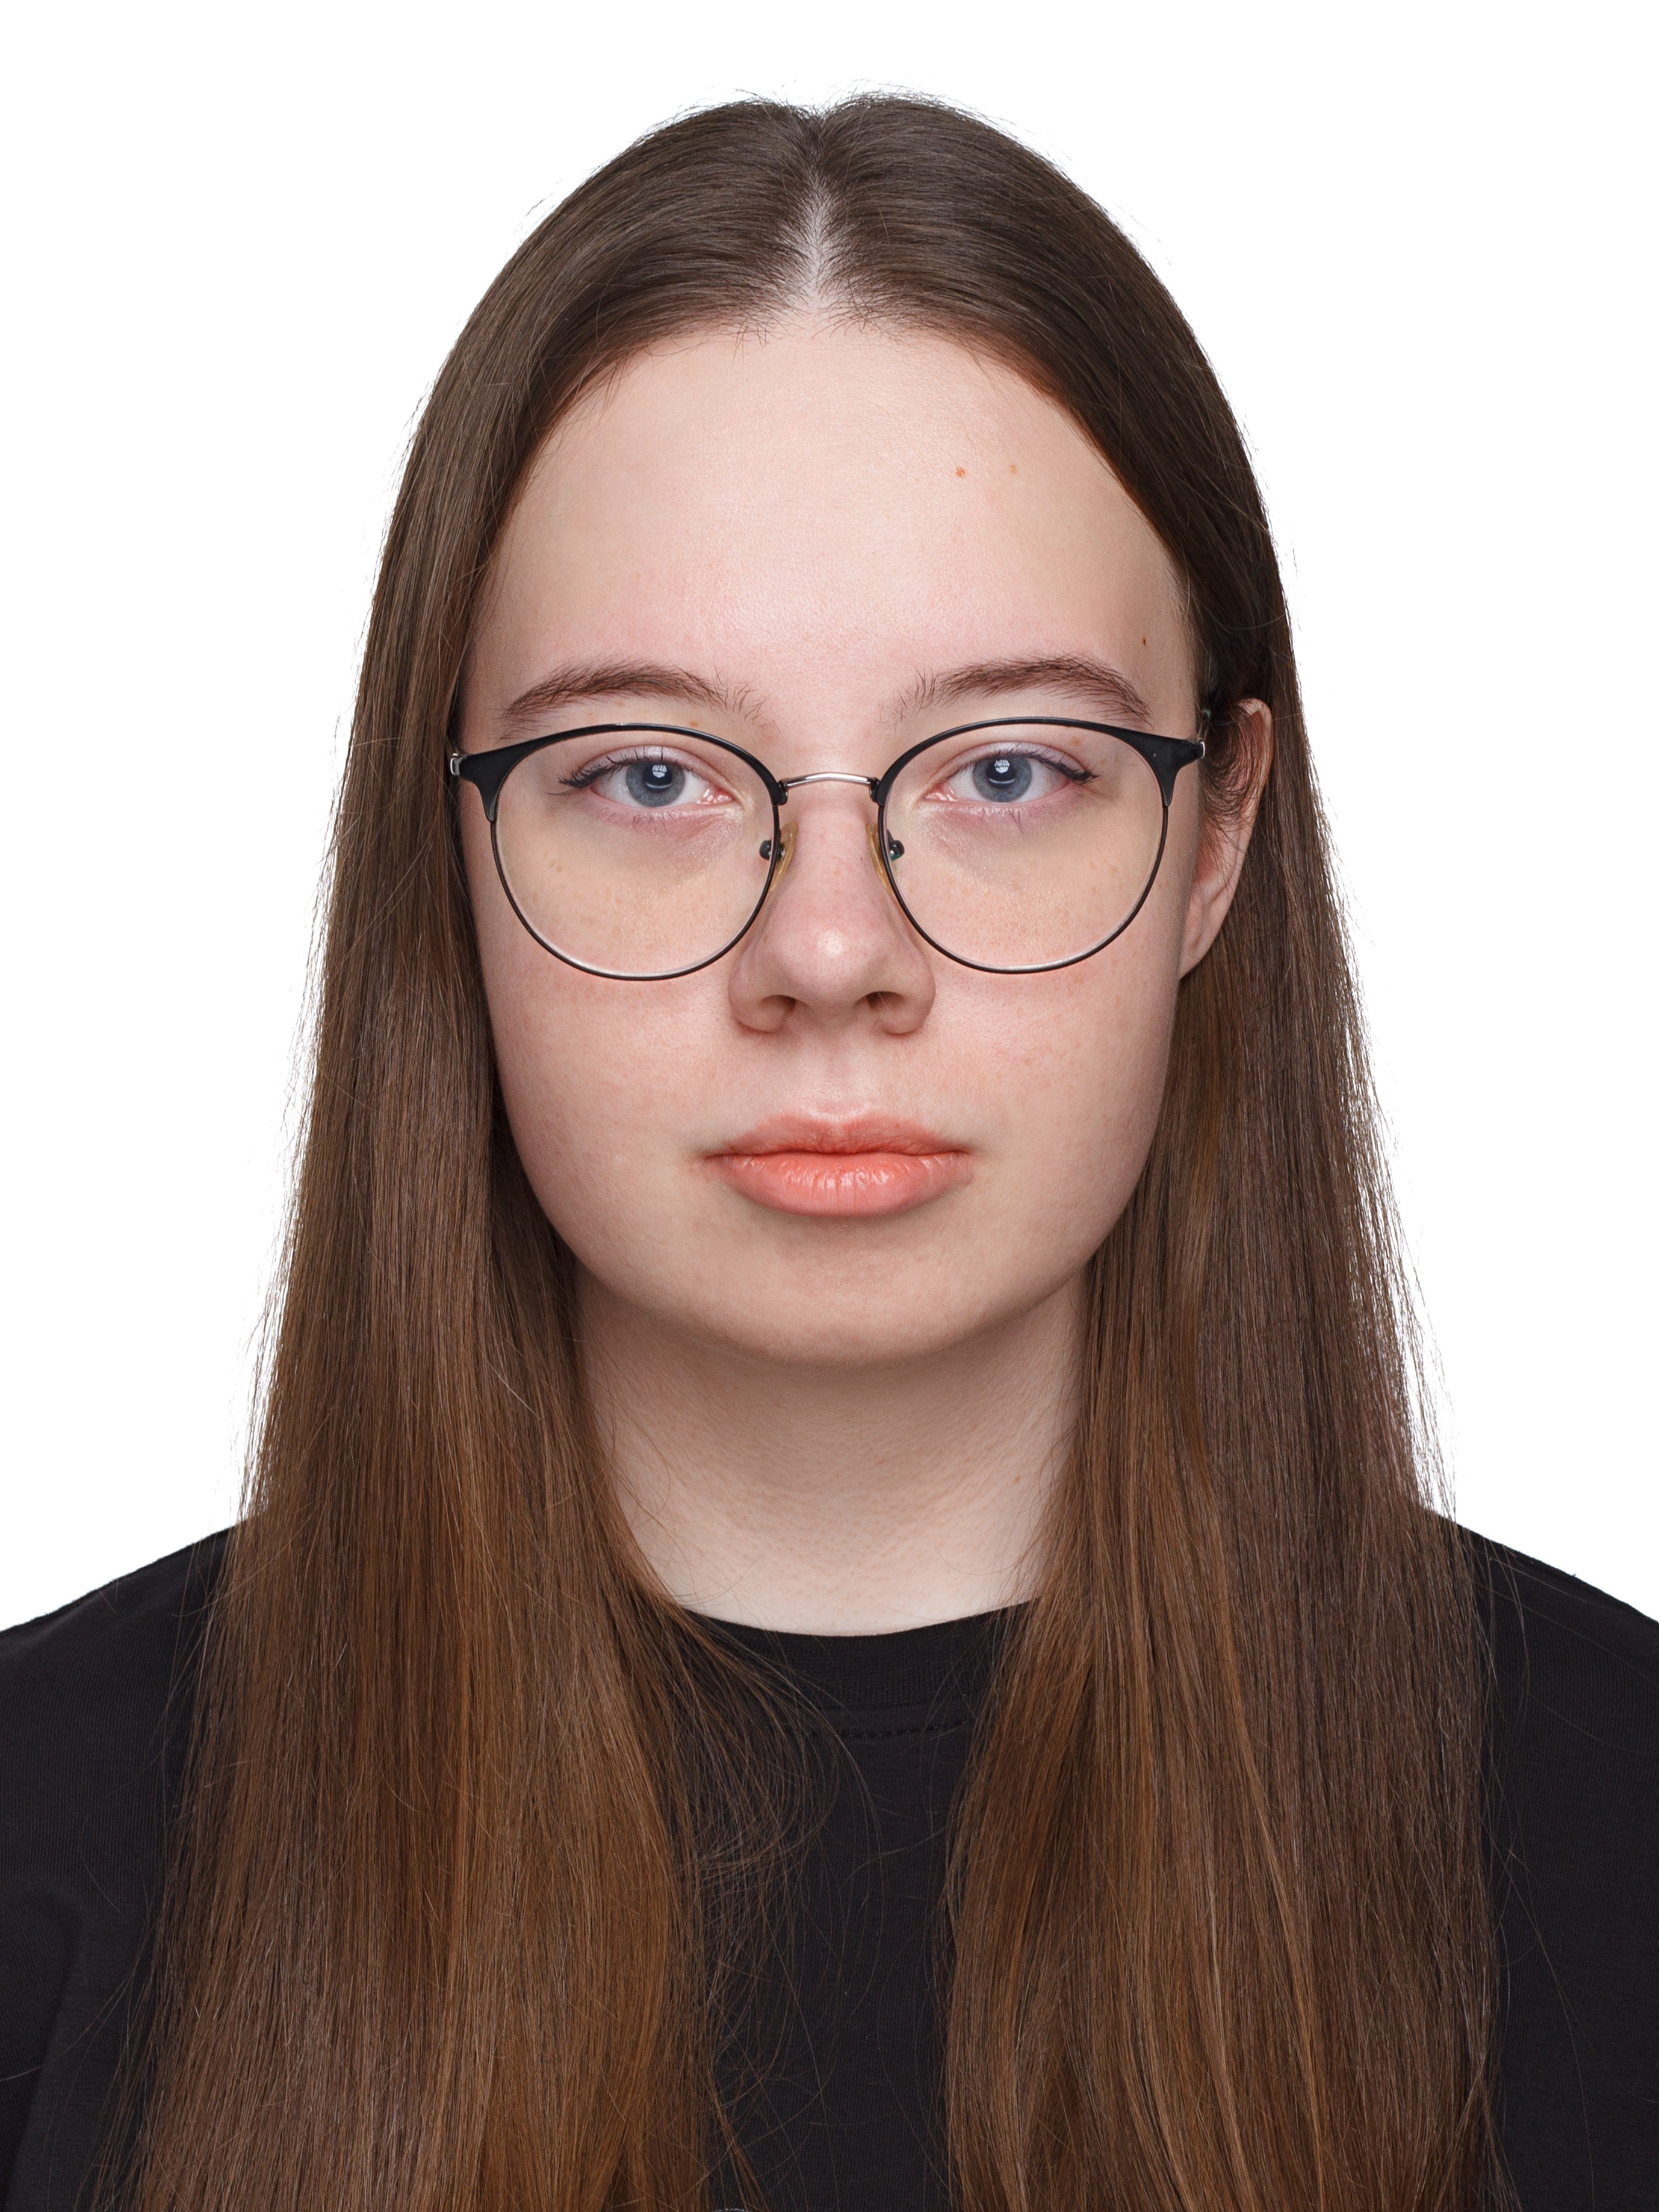
\includegraphics[width=0.6\linewidth]{photo.jpg}
  \end{minipage}%
  \par\vspace{8pt}%
}

\begin{document}
\pagestyle{empty}

\cvheader
\vspace{4pt}

\begin{multicols*}{2}

\cvsection{Образование}

\noindent\textbf{Университет Иннополис}\hfill 2023--2027\par
\vspace{2pt}
\noindent{бакалавриат «Анализ данных и искусственный интеллект»}\par
\vspace{2pt}
\noindent -- средний балл 4.8\par
\vspace{4pt}

\cvsection{Связанные курсы}

\noindent\textbf{Базы данных}~--- проектирование схем, SQL, нормализация, транзакции\par
\noindent\textbf{Введение в девопс}~--- CI/CD, Docker, автоматизация сборки и развёртывания\par
\noindent\textbf{Компьютерные сети}~--- модель OSI, TCP/IP, протоколы, маршрутизация\par
\noindent\textbf{Компьютерная архитектура}~--- устройство процессора, память, архитектура фон Неймана\par
\noindent\textbf{Создание прикладного проекта}~--- полный цикл разработки ПО: от требований до продукта\par

\cvsection{Навыки}

\cvskill{SQL и базы данных:}{PostgreSQL, MySQL, проектирование БД, оптимизация запросов}
\cvskill{Системный анализ:}{сбор требований, Use Cases, BPMN, UML, описание границ систем}
\cvskill{Процессы и инструменты:}{Git, Docker, Linux, CI/CD, Scrum, Kanban, REST API}
\cvskill{Безопасность и архитектура:}{основы безопасности ПО, SDLC, взаимодействие систем}

\cvsection{Английский язык}

\noindent\textbf{Professional}~--- разговорный, письменный, техническая литература, академический английский\par

\cvsection{Опыт работы}

\cvjob{Системный аналитик InNoHassle}{%
  \href{https://github.com/one-zero-eight}{one-zero-eight}, 2024 г.~--- наст. время}{%
  работаю в команде \href{https://innohassle.ru/}{InNoHassle} (500+ уникальных пользователей в день): собираю и формализую требования, описываю границы системы и пользовательские сценарии, проектирую взаимодействие компонентов, перевожу бизнес-потребности в технические спецификации для разработки.}

\cvjob{Специалист}{%
  \href{https://innopolis.university/}{Университет Иннополис}, окт. 2024~-- окт. 2025}{%
  возглавила процесс автоматизации составления расписания занятий в университете: ручной труд был заменён на программу, что сократило время составления расписания и практически исключило ошибки.}

\newcolumn

\cvsection{Проекты}

\cvproject{Системный анализ InNoHassle}{https://innohassle.ru/}{%
  описала пользовательские сценарии и границы системы, формализовала требования к улучшениям, построила модель приоритизации задач по влиянию на бизнес-метрики и пользовательский опыт}{%
  системный анализ, сбор требований, описание границ системы, BPMN, пользовательские сценарии}

\cvproject{Прогнозирование тяжести ДТП}{https://github.com/Big-Data-IU/US-Accidents}{%
  спроектировала схему данных и витрины для 7.7 млн записей, построила ETL-пайплайн, провела SQL-анализ факторов ДТП и описала взаимодействие компонентов системы}{%
  PostgreSQL, проектирование БД, Spark SQL, PySpark, Superset, ETL}

\cvproject{Автоматизация пайплайна аналитики}{https://github.com/belyakova-anna/Extrovert-vs.-Introvert-Predictor-Part-2}{%
  спроектировала пайплайн обработки данных, провела анализ признаков и автоматизировала процесс предсказаний: от загрузки данных до финального отчёта}{%
  Python, pandas, Airflow, проектирование пайплайнов, автоматизация}

\cvproject{Моделирование данных закупок}{https://github.com/one-zero-eight/hackathon-tenderhack}{%
  разработала модель объединения товарных позиций, кластеризовала дубликаты и построила карточки продуктов для аналитики закупочных процессов}{%
  Python, проектирование модели данных, векторизация, Qdrant}

\cvsection{Хакатоны}

\noindent\href{https://drive.google.com/file/d/1jkN7tX9rNNIsZIB6O6MDiqZsnLEl27lU/view?usp=sharing}{\textcolor{linkblue}{Победитель}} хакатона Tender Hack Казань\par
\noindent\href{https://drive.google.com/file/d/1EoGAExuRGV5qIiCAShXfYlCXQAhdUN0J/view?usp=sharing}{\textcolor{linkblue}{Призёр}} хакатона Tender Hack Санкт-Петербург\par
\noindent\href{https://drive.google.com/file/d/1BWFGwSSAwSdn6s5EZF81ADpFYrGgGW7c/view?usp=sharing}{\textcolor{linkblue}{Призёр}} хакатона Архипелаг\par
\noindent Участник: \href{https://drive.google.com/file/d/1F9VDEHMKZnxWCKisxFfVjK9pFhIeqrVx/view?usp=sharing}{Внедрейд}, \href{https://drive.google.com/file/d/1qB8kDuc\_pAsapLfi0IzUPYvbemiUm92D/view?usp=sharing}{True Tech Hack}, \href{https://drive.google.com/file/d/16w7wOoZbr\_ehW2p4fDqZiwhhCTPKn453/view?usp=sharing}{VTB More Tech}, \href{https://drive.google.com/file/d/1rXyqXFqTrNMfYjYB09TvNKFCe8gF2RKY/view?usp=sharing}{Tender Hack Пермь}\par

\cvsection{Достижения}

\noindent\textbf{Член сборной} Республики Татарстан по обработке изображений с БАС\par
\textbf{Член сборной} Республики Марий Эл по спортивному программированию\par
\noindent\textbf{Студент года} Университета Иннополис\par
\textbf{Финалист} Баттла Вузов\par

\end{multicols*}

\end{document}
